\section{Denoise Diffusion Probabilistic Models (DDPMs)}


\subsection{Diffusion Models (DMs)}
\label{subsec:diffusion_models}

Diffusion models are probabilistic generative models that map latent variables to observed data. Unlike GANs, they are easier to train and can produce high-quality images by progressively adding and removing noise. Most importantly, this model serves as a basis to other generative models.

A diffusion model consists of:

\begin{itemize}
    \item An encoder that maps the data $x$ through stochastic intermediate latent variables $z_1, ..., z_T$.
    \item And a decoder reversing the noising process
\end{itemize}








\subsection{DDPMs}
\label{sec:ddpm}

Denoise Diffusion Probabilistic Models (DDPMs) \cite{ddpm} are a class of diffusion models that are trained to denoise images by reconstructing a noised image. 

There are two processes, each process takes multiple ($t$) steps:

\begin{itemize}
    \item \textbf{Forward diffusion process}: Adds noise to the input image\footnote{There are multiple implementations on how to add noise to image. The simplest way is to use random values for each pixel (\texttt{torch.randn\_like()}) by tensor addition, but the most common way is to use Gaussian noise which distributes the noise normally (\texttt{np.random.normal(mean, sigma, ...)}).}. The addition of noise is the addition of random pixel values to the input image. In forward diffusion, we transform the image $x$ (from the dataset, without noise) to a latent variable $z_0 = x$. Then we add noise to get $z_1$, and so on, until $t$ steps we get $z_t$ - which is pure noise image, distributed from the noise distribution (usually Gaussian). The forward diffusion step is denoted as $\mathbf{q(x_t | x_{t-1})}$.
    
    \item \textbf{Reverse diffusion process}: Removes noise from the input noised image. The removal of noise can be thought as adding new features to the image. In reverse diffusion, we transform the image $z_t$ to $z_{t-1}$ by removing noise in a single step. We repeat this process until we get the original image $x = z_0$. The reverse diffusion step is denoted as $\mathbf{p_\theta (x_{t-1} | x_t)}$.
\end{itemize}

Because the addition of noise is a known stochastic process, \textbf{all the learned parameters are in the decoder} (the generator). We don't want to learn the addition of noise, since the task is to denoise the image. DDPMs learn with a fixed inference procedure $q(x_{1:T} | x_0)$.

DDPMs are latent variable models in the form of:

\begin{equation*}
    p_\theta (x_0) = \int p_\theta(x_{0:T}) dx_{1:T} \text{,\ \ where \ \ \ } p_\theta (x_{0:T}) := p_\theta (x_T) \prod_{t=1}^{T} p_\theta (x_{t-1} | x_t)
\end{equation*}

Because this \textbf{integral is intractable}, we use ELBO. The parameters of the model $\theta$ are learned to fit the data distribution $q(x_0)$ by \textbf{maximizing a variational lower bound}:

\begin{equation*}
    \max_{\theta} \mathbb{E}_{q(x_0)} [\log p_\theta (x_0)] \leq \max_\theta \mathbb{E}_{q(x_0, x_1, ..., x_T)} [\log p_\theta (x_{0:T}) - \log q(x_{1:T} | x_0)]
\end{equation*}

where $q(x_{1:T} | x_0)$ is the reverse diffusion process over the latent variables.


\begin{figure}
    \centering
    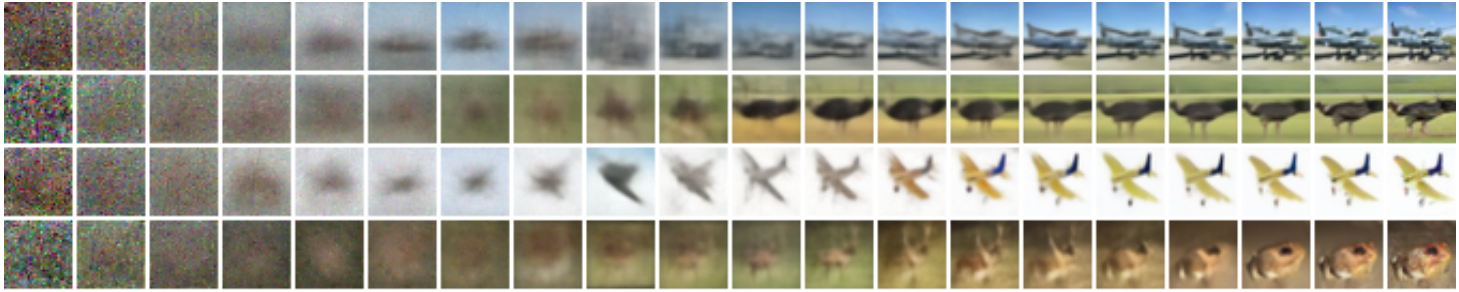
\includegraphics[width=1\textwidth]{images/diffusion_models/ddpm_denoise.png}
    \caption{Progressive generation (left to right) of unconditional CIFAR10 dataset in DDPM \cite{ddpm}.}
\end{figure}


\begin{figure}
    \centering
    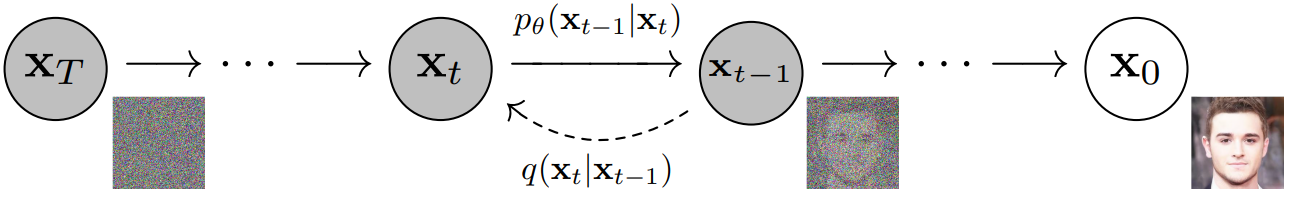
\includegraphics[width=0.7\textwidth]{images/diffusion_models/ddpm_process.png}
    \caption{A graph representing the forward ($q(x_t | x_{t-1})$) and reverse ($p_\theta(x_{t-1} | x_t)$) diffusion process in DDPMs \cite{ddpm}. The next step (either in forward or reverse diffusion) depends conditionally on the previous steps (Markov chains) \cite{ddpm}.}
    \label{fig:ddpm_process}
\end{figure}






\begin{figure}[h]
    \centering
    \begin{minipage}{0.10\textwidth}
        \centering
        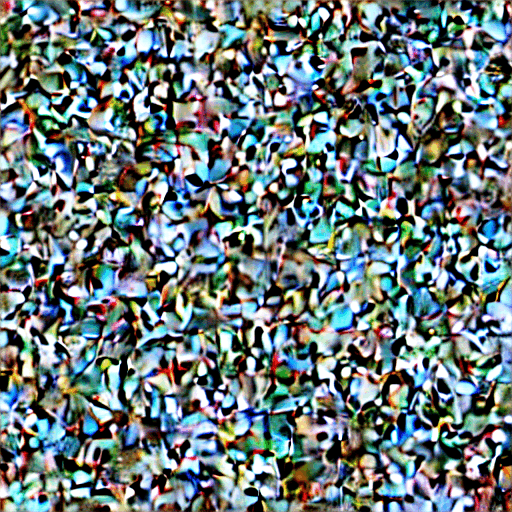
\includegraphics[width=\textwidth]{images/diffusion_models/noise_to_image_gif/0.png}
    \end{minipage}
    \begin{minipage}{0.10\textwidth}
        \centering
        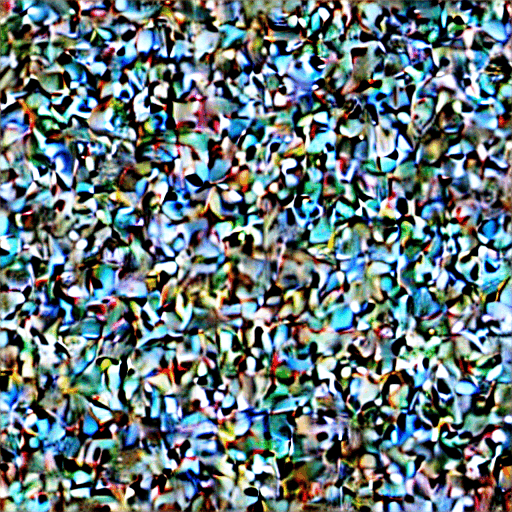
\includegraphics[width=\textwidth]{images/diffusion_models/noise_to_image_gif/1.png}
    \end{minipage}
    \begin{minipage}{0.10\textwidth}
        \centering
        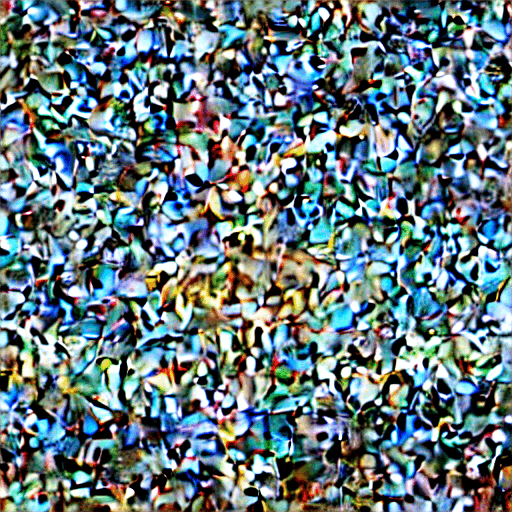
\includegraphics[width=\textwidth]{images/diffusion_models/noise_to_image_gif/2.png}
    \end{minipage}
    \begin{minipage}{0.10\textwidth}
        \centering
        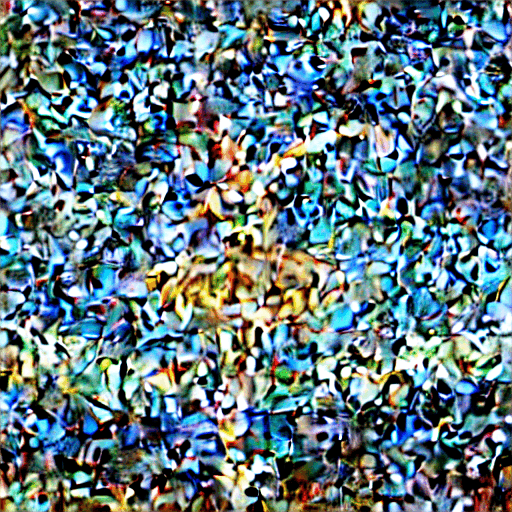
\includegraphics[width=\textwidth]{images/diffusion_models/noise_to_image_gif/3.png}
    \end{minipage}
    \begin{minipage}{0.10\textwidth}
        \centering
        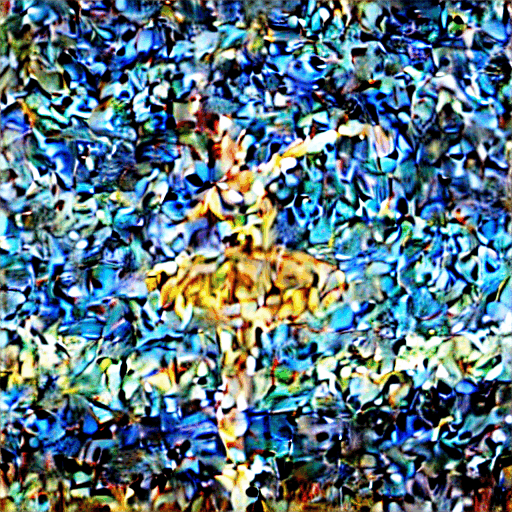
\includegraphics[width=\textwidth]{images/diffusion_models/noise_to_image_gif/4.png}
    \end{minipage}
    \begin{minipage}{0.10\textwidth}
        \centering
        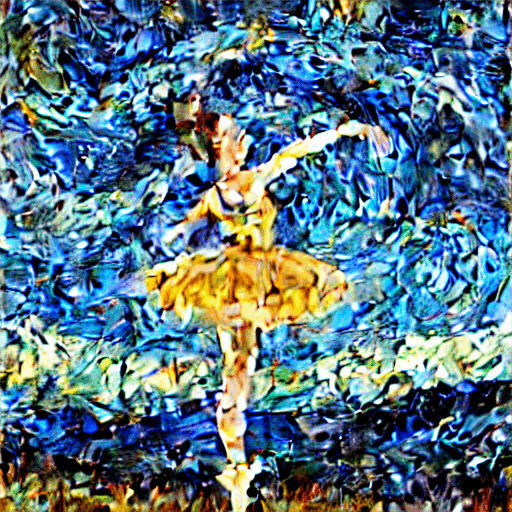
\includegraphics[width=\textwidth]{images/diffusion_models/noise_to_image_gif/5.png}
    \end{minipage}
    \begin{minipage}{0.10\textwidth}
        \centering
        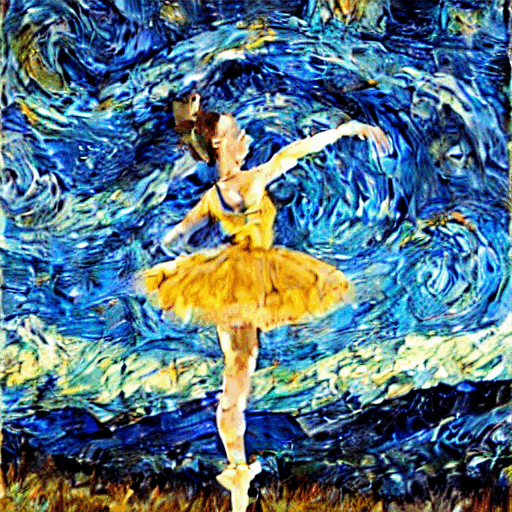
\includegraphics[width=\textwidth]{images/diffusion_models/noise_to_image_gif/6.png}
    \end{minipage}
    \begin{minipage}{0.10\textwidth}
        \centering
        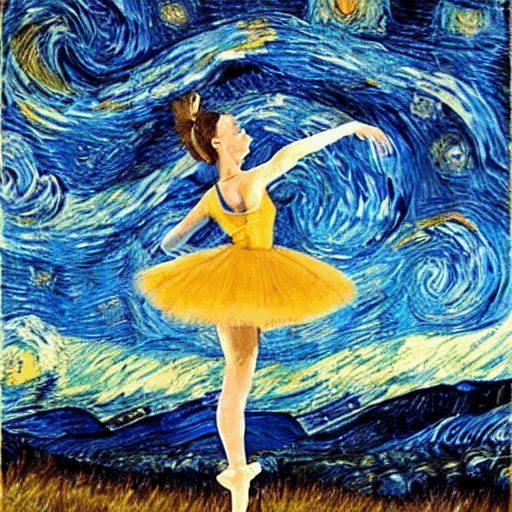
\includegraphics[width=\textwidth]{images/diffusion_models/noise_to_image_gif/7.png}
    \end{minipage}
    \caption{Progressive denoising of latents in DDPM. Images taken from the \href{https://scholar.harvard.edu/binxuw/classes/machine-learning-scratch/materials/stable-diffusion-scratch}{harvard university} website.}
\end{figure}






\subsection{Noise Schedulers}

A noise scheduler defines how noise is added to the image at each timestep (for the forward process in DDPMs). Instead of adding noise all at once, a scheduler defines how much noise to add periodically (in steps).

Typically, we control noise schedulers with two parameters: $\alpha_t$ which controls how much noise is added (strength of the noise) at step $t$, and $\beta_t$ which controls the variance  of the noise added at step $t$ (typically referred to as just 'noise schedule' or 'variance').

In the paper \cite{ddpm} the authors used linear scheduler, however OpenAI released a paper \cite{openai_improved_ddpm} that uses cosine scheduler. They have shown that a cosine scheduler performs better than a linear scheduler in terms of image generation quality (see figure \ref{fig:linear_cosine_scheduler}).

\begin{figure}
    \centering
    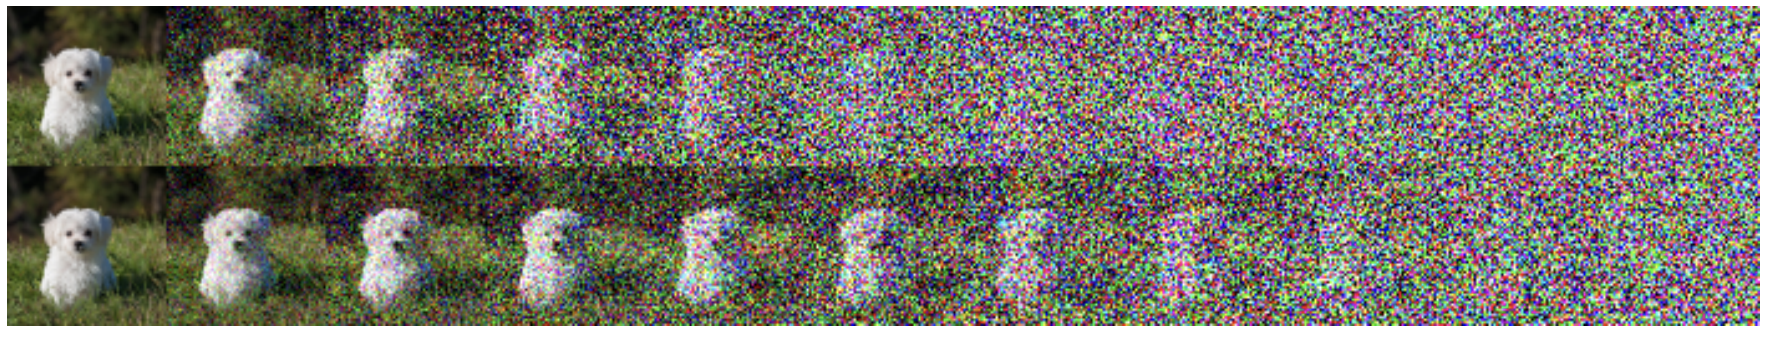
\includegraphics[width=1\textwidth]{images/diffusion_models/linear_cosine_scheduler.png}
    \caption{\textit{Top}: Linear scheduler \cite{ddpm}; \textit{Bottom}: cosine scheduler \cite{openai_improved_ddpm}. The linear scheduler adds noise too quickly which degrades the model's performance quickly, whereas cosine scheduler adds noise more slowly \cite{openai_improved_ddpm}.}
    \label{fig:linear_cosine_scheduler}
\end{figure}

A variance schedule is simply a function that defines the variance at each given timestep during the forward diffusion process. At each timestep, Gaussian noise $\epsilon$ is added to the previous latent variable:

\[
    x_{t+1} = \sqrt{1 - \beta_t} x_t + \sqrt{\beta_t} \epsilon
\]

Notice that when $\beta$ increases linearly, the term $\sqrt{1-\beta}$ decreases linearly. 

A noise scheduler is a function: $\beta(t):[1, ..., T] \rightarrow \mathbb{R}$ that determines the amount of noise added at each step. Its a sequence of $\alpha_t$.

A \textbf{linear scheduler} \textbf{linear scheduler} is defined as:
\[
    \beta_t = c \cdot t \text{, where c is constant}
\]

and a \textbf{cosine-beta scheduler} can be defined as:

\[
    \bar{\alpha}_t = \frac{f(t)}{f(0)} \text{, where } f(t) = \cos^2 \left( \frac{t/T + s}{1+s} \cdot \frac{\pi}{2} \right)
\]








\subsection{Encoder}

The forward diffusion process maps a data image $x$ through a series of intermediate variables $z_1, ..., z_T$ with the dimension as $x$ according to the following recursion:

\begin{equation}
    \begin{aligned}
    \mathbf{z}_1 &= \sqrt{1 - \beta_1} \cdot \mathbf{x} + \sqrt{\beta_1} \cdot \epsilon_1, \\
    &\;\;\vdots \notag \\
    \mathbf{z}_t &= \sqrt{1 - \beta_t} \cdot \mathbf{z}_{t-1} + \sqrt{\beta_t} \cdot \epsilon_t \quad \forall \, t \in \{2, \ldots, T\}
    \end{aligned}
\end{equation}

At each step $i \in \{1, 2, ..., t, t+1, ..., T\}$ a noise vector $\epsilon_i$ is drawn from a standard normal distribution. This equation adds random noise $\epsilon_i$ to the image $x = z_0$ and $\beta$ is a schedule function ($\beta(t):[1, ..., T] \rightarrow \mathbb{R}$) that determines the amount of noise added at each step ($\beta$ is a variance schedule, which can be linear, cosine, quadratic and more). 

A more formal notation for the \textbf{forward diffusion process} is:

\begin{equation*}
    \begin{aligned}
        q(x_t | x_{t-1}) = \mathcal{N}(x_t; \sqrt{1-\beta_t} \cdot x_{t-1}, \beta_t \mathbf{I}) \\
        q(x_{1:T} | x_0) = \prod_{t=1}^{T} q(x_t | x_{t-1})
    \end{aligned}
\end{equation*}

\begin{itemize}
    \item The noise is sampled from a normal distribution $\epsilon \sim \mathcal{N}(0, 1)$.
    \item The latent variable $x_t$ is sampled from a normal distribution $\mathcal{N}$ where:
    \begin{itemize}
        \item The mean is $\sqrt{1-\beta_t} \cdot x_{t-1}$.
        \item The variance is $\beta_t \mathbf{I}$.
        \item The $\beta$ parameter is the noise scheduler (how much noise we add at each step).
    \end{itemize}
\end{itemize}



\subsubsection*{Skipping intermediate steps in forward diffusion}


An interesting point the authors made is that in forward diffusion it is possible to sample $x_t$ from any arbitrary timestep $t$, given the original image $x_0$ (without calculating all the intermediate steps):

\begin{equation}
    \begin{aligned}
    q(\mathbf{x}_t|\mathbf{x}_0) = \mathcal{N}(\mathbf{x}_t; \sqrt{\bar{\alpha}_t}\mathbf{x}_0, (1 - \bar{\alpha}_t)\mathbf{I}) \\
    \text{where } \alpha_t := 1 - \beta_t \text{ and } \bar{\alpha}_t := \prod_{i=1}^{t} \alpha_i
    \end{aligned}
    \label{eq:forward_diffusion}
\end{equation}

Since $\alpha$ depends on $\beta$ we can see that \textbf{there are no parameters to learn in the forward diffusion process}.

After plugging in $\alpha = 1 - \beta$ in the encoder and the \textbf{reparametrization trick} (from VAE: $\mathcal{N} (\mu, \sigma^2) = \mu + \sigma \cdot \epsilon \text{, where } \epsilon \sim \mathcal{N}(0, 1) $) we get:

\begin{align*}
    q(x_t | x_{t-1}) &= \mathcal{N} \left( x_t; \sqrt{1-\beta_t} x_{t-1}, \beta_t \mathbf{I} \right) \\
    &= \sqrt{1-\beta_t} x_{t-1} + \sqrt{\beta_t} \epsilon_t \\
    &= \sqrt{\alpha_t} x_{t-1} + \sqrt{1 - \alpha_t} \epsilon \\
    &= \sqrt{\alpha_t \alpha_{t-1}} x_{t-2} + \sqrt{1 - \alpha_t \alpha_{t-1}} \epsilon \\
    &= \sqrt{\alpha_t \alpha_{t-1} \alpha_{t-2}} x_{t-3} + \sqrt{1 - \alpha_t \alpha_{t-1} \alpha_{t-2}} \epsilon \\
    &= \sqrt{\alpha_t \alpha_{t-1} \cdots \alpha_1 \alpha_0} x_0 + \sqrt{1 - \alpha_t \alpha_{t-1} \cdots \alpha_1 \alpha_0} \epsilon \\
    &= \boxed{ \sqrt{\bar{\alpha}} x_0 + \sqrt{1 - \bar{\alpha}} \epsilon }
\end{align*}

as a result we get:

\begin{equation}
    q(x_t | x_0) = \mathcal{N} (x_t; \sqrt{\bar{\alpha_t}} x_0, (1-\bar{\alpha_t}) \mathbf{I})
    \label{eq:forward_diffusion_single_step}
\end{equation}

Equation \ref{eq:forward_diffusion_single_step} describes how in a single step we can get a noisier image $x_t$ from the original image $x_0$ without calculating all the intermediate steps. This is a very useful property of latent diffusion models.









\subsection{Decoder}

The decoder removes noise from the intermediate latent variables $z_T, ..., z_1$ and reconstructs the original image $x = z_0$ using the following recursion:

\begin{equation}
    p_\theta(\mathbf{x}_{t-1} | \mathbf{x}_t) = \mathcal{N}(\mathbf{x}_{t-1}; \mu_\theta(\mathbf{x}_t, t), \Sigma_\theta(\mathbf{x}_t, t))
    \label{eq:reverse_diffusion}
\end{equation}

where $\theta$ are the learned parameters of the model. The mean $\mu_\theta$ and variance $\Sigma_\theta$ are unknown and should be learned in the training. 


\subsubsection*{Learning the variance}

In the DDPM paper \cite{ddpm} the authors said:

\begin{quote}
    \textit{"We also see that learning reverse process variances (by incorporating a parameterized diagonal $\Sigma_\theta(x_t)$ into the variational bound) leads to unstable training and poorer sample quality compared to fixed variances."} \cite{ddpm}
\end{quote}

The OpenAI team released a paper titled "Improved denoising diffusion probabilistic models" \cite{openai_improved_ddpm} in which the authors used cosine noise (instead of linear in the original paper \cite{ddpm}) scheduler and also \textbf{learned the variance}, which significantly improved the model's performance.








\subsection{Loss function}

Diffusion models are in the form of $p_\theta (x_0) := \int p_\theta(x_{0:T}) d\mathbf{x}_{1:T}$ which is intractable, thus we use the ELBO loss function to approximate the likelihood of the data.

We seek to train the model to predict the noise $\epsilon_i$ added at each timestep. We could start with a simple loss function (\textbf{negative log likelihood}):

\[ -\log (p_\theta (x_0)) \]

but that's a problem, the probability of $x_0$ depends on all timesteps $x_0, x_1, ..., x_T$. As a solution, loss function of DDPMs is typically the \textbf{variational lower bound} of this objective:

\[
    -\log (p_\theta(x_0)) \leq -\log (p_\theta(x_0)) + D_{KL} (q(x_{1:T} | x_0)) \vert \vert p_\theta(x_{1:T} | x_0)
\]

We can rewrite the KL-divergence as \footnote{Thanks in part for the math explanation to \href{https://www.youtube.com/watch?v=HoKDTa5jHvg}{a youtube video that explained the math in the paper}.}:

\begin{align*}
    D_{KL} (q(x_{1:T} | x_0)) \vert \vert p_\theta(x_{1:T} | x_0) &= \log(\frac{q(x_{1:T} | x_0)}{p_\theta(x_{1:T} | x_0)}) \\
    &= \log(\frac{q(x_{1:T} | x_0)}{ \frac{p_\theta(x_0 | x_{1:T}) p_\theta(x_{1:T})}{p_\theta(x_0)} }) \\
    &= \log(\frac{q(x_{1:T} | x_0)}{ \frac{p_\theta(x_0, x_{1:T})}{p_\theta(x_0)} }) \\
    &= \log(\frac{q(x_{1:T} | x_0)}{ \frac{p_\theta(x_{0:T})}{p_\theta(x_0)} }) \\
    &= \log(\frac{q(x_{1:T} | x_0)}{ p_\theta(x_{0:T}) }) + \log(p_\theta(x_0))
\end{align*}

By reformulating the KL-divergence we arrive at the following loss objective (the terms $-\log(p_\theta(x_0))$ and $\log(p_\theta(x_0))$ cancel each other out):

\begin{align*}
    -\log (p_\theta(x_0)) &\leq -\log (p_\theta(x_0)) + \log (\frac{ q(x_{1:T} | x_0) }{ p_\theta (x_{0:T}) }) + \log(p_\theta(x_0)) \\
    &= \log (\frac{ q(x_{1:T} | x_0) }{ p_\theta (x_{0:T}) }) \\
\end{align*}

we finally get the \textbf{variational lower bound (ELBO)}:

\[
\begin{tikzcd}
    \textcolor{green}{-\log(p_\theta(x_0))} \leq \log(\frac{\textcolor{red}{q(x_{1:T} | x_0)}}{\textcolor{blue}{p_\theta(x_{0:T})}})
    \arrow[d, ""] \\
    \boxed{
        \mathcal{L} = 
        \underbrace{\mathbb{E}[
            \textcolor{green}{-\log p_\theta (x_0)}
        ] }_{\text{NLL}}
        \leq 
        \underbrace{\mathbb{E}_q[-\log (\frac{
            \textcolor{blue}{p_\theta(x_{0:T})}
        }{
            \textcolor{red}{q(x_{1:T}|x_0)}})]}_{\text{ELBO}
        }
    }
\end{tikzcd}
\]

The dominator $\textcolor{red}{q(x_{1:T}|x_0)}$ is the forward diffusion process (adds noise) and the numerator $\textcolor{blue}{p_\theta(x_{0:T})}$ is the reverse process. 

The ratio of these two terms is the ELBO loss function and when this ratio reaches 1, it indicates that the model can undo the forward process. We also don't write $q_\theta$ because the forward process is not learned, only the reverse process is learned.

We can simplify the training objective of DDPMs as simply \textbf{noise predictor} - commonly written as $\epsilon$-prediction:

\begin{equation}
    \boxed{\mathcal{L}_\text{simple} (\theta) = \mathbb{E}_{t,x_0, \epsilon} \left[ \left| \left| \epsilon - \epsilon_\theta (x_t, t) \right| \right|^2 \right]}
    \label{eq:ddpm_loss}
\end{equation}

where $\epsilon_\theta (x_t, t)$ is the noise predicted by the model, given timestep $t$ and noisy input $x_t$.







\subsection{Training}

The training of diffusion models is done by sampling a batch of images from the dataset, and then adding noise to the images in the forward diffusion process. The model is trained to remove the noise and reconstruct the original image in the reverse diffusion process. The loss function is the ELBO loss function. Usually, the model is trained using stochastic gradient descent (SGD), but more advanced optimizers like Adam can be used as well.





\begin{algorithm}
    \caption{The training algorithm of diffusion models \cite{ddpm}.}
    \label{alg:ddpm_training}
    \begin{algorithmic}[1] % Enables line numbering
        \State \textbf{repeat}
        \State \hspace{5pt} $ \mathbf{x}_0 \sim q(\mathbf{x}_0) $
        \State \hspace{5pt} $ t \sim \text{Uniform}(\{1, \dots, T\}) $
        \State \hspace{5pt} $ \epsilon \sim \mathcal{N}(\mathbf{0}, \mathbf{I}) $
        \State \hspace{5pt} Take gradient descent step on
        \[
        \nabla_{\theta} \left\| \epsilon - \epsilon_{\theta} \left( \sqrt{\bar{\alpha}_t} \mathbf{x}_0 + \sqrt{1 - \bar{\alpha}_t} \epsilon, t \right) \right\|^2
        \]
        \State \textbf{until} converged
    \end{algorithmic}
\end{algorithm}





In algorithm \ref{alg:ddpm_training} line 2, we take a sample from the dataset. In line 3, we generate random number between 1 and T uniformly. In line 4, we sample some noise. Line 5: we calculate the gradients of the loss function: we try to optimize the model's parameters $\theta$ by gradient decent. $\epsilon_\theta$ is the predicted noise added at timestep $t$ (a function approximator with 2 parameters that intends to predict $\epsilon$ from $x_t$) where the first parameter is the noisy image at timestep $t$, and the second parameter is the timestep $t$.



